\documentclass[11pt,a4paper]{article}
\usepackage[left=24mm,right=24mm,top=20mm,bottom=20mm,headheight=14pt]{geometry}
\usepackage[T1]{fontenc}
\usepackage{lmodern}
\usepackage{microtype}
\usepackage{amsmath,amssymb,amsthm}
\usepackage{graphicx}
\graphicspath{{../paper/figures/}{../thermal-feedback/figures/}}
\usepackage{booktabs}
\usepackage{fancyhdr}
\usepackage{xcolor}
\usepackage{tikz}
\usetikzlibrary{arrows.meta}
\usepackage[colorlinks=true,linkcolor=blue!50!black,citecolor=blue!50!black,urlcolor=blue!50!black]{hyperref}
\usepackage{caption}
\captionsetup{font=small,labelfont=bf}
\setlength{\parindent}{1.5em}
\setlength{\parskip}{0pt}
\setlength{\textfloatsep}{12pt plus 2pt minus 2pt}
\setlength{\intextsep}{12pt plus 2pt minus 2pt}
\pagestyle{fancy}
\fancyhf{}
\fancyhead[L]{\small Stability of the Hawking--Bondi balance}
\fancyhead[R]{\small E. Anaraly uulu}
\fancyfoot[C]{\thepage}
\renewcommand{\headrulewidth}{0.3pt}
\newtheorem{proposition}{Proposition}
\newcommand{\Pbb}{P_{\mathrm{bb}}}
\newcommand{\Mcrit}{M_{\mathrm{crit}}}
\newcommand{\Mc}{M_{c0}}
\newcommand{\tstar}{t_*}
\newcommand{\taubb}{\tau_{\mathrm{bb}}}
\newcommand{\Cenv}{C_{\mathrm{env}}}

\begin{document}
\begin{center}
{\LARGE\bfseries Can a Microscopic Black Hole\\[2pt] Be Held at Constant Mass?\par}
\vspace{5pt}
{\large Stability of the Hawking--Bondi balance in fixed and thermally coupled media\par}
\vspace{13pt}
{\normalsize Emir Anaraly uulu\par}
Independent Researcher, Bishkek, Kyrgyz Republic\\
\href{mailto:anarem1004@gmail.com}{\texttt{anarem1004@gmail.com}}\\[7pt]
First manuscript: 10 May 2026 \quad\textbar\quad This version: 22 October 2026
\end{center}
\vspace{4pt}

\begin{abstract}
A microscopic black hole loses mass by Hawking evaporation and can regain it by accreting the surrounding gas. We ask whether the two processes can hold its mass constant. Combining idealized Bondi accretion with a blackbody approximation to Hawking emission, we first show that in a fixed medium the mass equation has exactly one positive balance and that this balance is unstable; an exact implicit solution gives the evaporation and growth times on either side. We then let the hole's radiation heat the medium. Coupling the mass to an effective gas temperature, with the Bondi rate scaling as $T^{-3/2}$ and linear cooling, yields a single hotter and more massive equilibrium whose Jacobian determinant is negative for every positive heating and cooling strength, so the equilibrium is a saddle. The result extends to any one-zone model in which heating decreases with mass, accretion decreases with temperature and cooling increases with temperature. Its origin is the sign of the feedback: unlike an accretion-powered source, a Hawking-powered hole radiates more as it loses mass, so heating suppresses accretion exactly when accretion is needed. Timescale estimates for two hydrogen plasmas show that neither supports the one-zone description at the balance mass. All results are reproducible from the accompanying code.
\end{abstract}

\section{Introduction}
Hawking radiation makes a black hole a heat source whose luminosity grows as its mass falls~\cite{hawking}. If surrounding matter replaced the evaporated mass, the hole might be held at a constant mass and radiate steadily. Whether such a state can exist is a question of stability: a balance between gain and loss is useful only if a small change in mass returns the system to it.

This study grew from an olympiad problem written for the Kyrgyz Republic national physics competition and used in IPhO-2026 team selection (Day~2, Problem~3, April 2026). The problem balanced Bondi accretion against Hawking evaporation for a hole in a fixed medium. Here we analyze that balance in full and then remove its strongest assumption, that the medium is unaffected by the hole's radiation.

The paper proceeds in two steps. In a fixed medium (Sec.~\ref{sec:fixed}), the mass obeys a single equation that we solve exactly; its only balance is unstable. Because a fixed medium ignores the hole's own heating, we then couple the mass to an effective temperature of the gas (Secs.~\ref{sec:model}--\ref{sec:numerics}). Heating moves the balance, and a recent hydrodynamic study shows that the thermodynamics of the inflowing gas can change the Bondi rate substantially~\cite{cantiello}; it is therefore not obvious in advance whether the feedback stabilizes or destabilizes. We prove that the coupled equilibrium is a saddle for all positive parameters, identify the physical reason, and extend the result to a class of monotone heating and cooling laws. Section~\ref{sec:physical} estimates whether any simple plasma could support the one-zone description.

Throughout, the black hole is uncharged and nonrotating, $M$ and $t$ refer to the asymptotic Schwarzschild description, and ``stability'' refers to the equilibria of the stated differential equations. Confinement, energy collection and engineering feasibility are outside the scope of this paper.

\section{Hawking emission and Bondi accretion}\label{sec:ingredients}
\subsection{Evaporation}
For a Schwarzschild black hole, the horizon radius and Hawking temperature are
\begin{equation}
 r_s=\frac{2GM}{c^2},\qquad T_H=\frac{\hbar c^3}{8\pi GMk_B}.
 \label{eq:temperature}
\end{equation}
Simple estimates (a Newtonian escape speed for $r_s$, the uncertainty principle for $T_H$) reproduce both scalings but not the coefficient of $T_H$; Appendix~\ref{app:temperature} derives it from the regularity of the Euclidean geometry~\cite{gibbons,genolini}. Treating the horizon, of area $4\pi r_s^2$, as a photon blackbody gives
\begin{equation}
 \Pbb=\frac{K}{M^2},\qquad K=\frac{\hbar c^6}{15360\pi G^2},\qquad
 \dot M_{\rm evap}=-\frac{B}{M^2},\qquad B=\frac{K}{c^2}.
 \label{eq:power}
\end{equation}
Numerically, $K=3.56\times10^{32}\,\mathrm{W\,kg^2}$ and $B=3.96\times10^{15}\,\mathrm{kg^3\,s^{-1}}$. At the reference mass $M_0=10^7$~kg used below, $T_H=1.23\times10^{16}$~K and $\Pbb=3.56\times10^{18}$~W. This photon blackbody is a simplified baseline. At $k_BT_H\simeq1$~TeV many particle species are emitted, and greybody factors modify each channel, so the true luminosity is larger~\cite{page,macgibbon}. All luminosities and lifetimes quoted below refer to the baseline.

\subsection{Accretion}
Steady spherical accretion of a polytropic gas at rest far from the hole proceeds at the Bondi rate~\cite{bondi}
\begin{equation}
 \dot M_{\rm acc}=AM^2,\qquad A=\frac{4\pi\lambda\rho_\infty G^2}{c_s^3},
 \label{eq:bondi}
\end{equation}
where $\rho_\infty$ and $c_s$ are the density and sound speed far from the hole and $\lambda=1/4$ for an adiabatic index $\gamma=5/3$. As a formal numerical reference for the fixed-medium model we take $\rho_\infty=10^3\,\mathrm{kg\,m^{-3}}$, $c_s=1500\,\mathrm{m\,s^{-1}}$ and $\lambda=1/4$, which gives $A=4.15\times10^{-27}\,\mathrm{kg^{-1}\,s^{-1}}$. These water-like values do not describe a polytropic gas, and the Bondi scale $r_B=GM/c_s^2$ is only $3\times10^{-10}$~m at $M_0$, comparable to molecular sizes; they serve to set numerical scales, not as a validated accretion model. Section~\ref{sec:physical} replaces them with ideal-gas plasmas.

\section{The fixed medium}\label{sec:fixed}
\subsection{A unique, unstable balance}
With $A$ and $B$ constant, the mass obeys
\begin{equation}
 \dot M=f(M)=AM^2-\frac{B}{M^2},\qquad M>0.
 \label{eq:mass}
\end{equation}
At $M_0$, accretion supplies $4.15\times10^{-13}\,\mathrm{kg\,s^{-1}}$ while evaporation removes $39.6\,\mathrm{kg\,s^{-1}}$. The two terms balance at a single mass,
\begin{equation}
 \Mcrit=\left(\frac BA\right)^{1/4},
 \label{eq:mcrit}
\end{equation}
which is unstable because
\begin{equation}
 f'(\Mcrit)=2A\Mcrit+\frac{2B}{\Mcrit^3}=4A\Mcrit>0.
 \label{eq:derivative}
\end{equation}
A slightly heavier hole accretes more and evaporates less, so it keeps growing; a slightly lighter hole does the opposite. Small perturbations grow as $e^{t/t_e}$ with $t_e=(4A\Mcrit)^{-1}$.

Measuring mass in units of $\Mcrit$ and time in units of $\tstar=(A\Mcrit)^{-1}$, with $x=M/\Mcrit$ and $s=t/\tstar$, every case with positive constant $A$ and $B$ reduces to
\begin{equation}
 \frac{dx}{ds}=x^2-x^{-2},
 \label{eq:dimensionless}
\end{equation}
whose fixed point $x=1$ has growth rate 4 (Fig.~\ref{fig:fixed-rate}). Changing the medium rescales $\Mcrit\propto(c_s^3/\rho_\infty)^{1/4}$ but cannot change the sign of $f'(\Mcrit)$.

\begin{figure}[tbp]
 \centering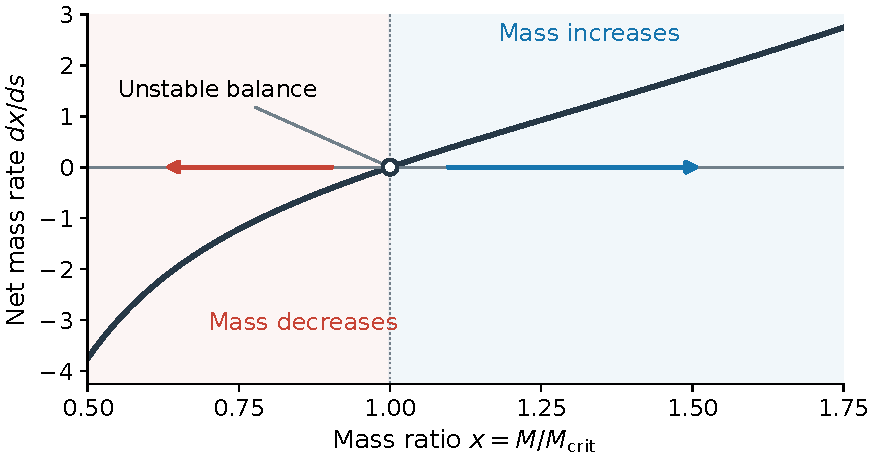
\includegraphics[width=.82\linewidth]{figure1.pdf}
 \caption{\textbf{Equal rates do not restore the mass.} The net dimensionless mass rate of Eq.~\eqref{eq:dimensionless} crosses zero at $x=1$ with positive slope, so masses on either side move away from the balance. The curve applies to every $A,B>0$.}
 \label{fig:fixed-rate}
\end{figure}

\subsection{Exact evolution}
Separating Eq.~\eqref{eq:dimensionless} and using partial fractions,
\begin{equation*}
 \frac{x^2}{x^4-1}=\frac12\left(\frac1{x^2-1}+\frac1{x^2+1}\right),\qquad
 F(x)=\frac14\ln\left|\frac{x-1}{x+1}\right|+\frac12\arctan x,
\end{equation*}
gives the exact implicit trajectory from an initial ratio $x_0$,
\begin{equation}
 s=F(x)-F(x_0).
 \label{eq:implicit}
\end{equation}
Mass decreases for $0<x_0<1$ and increases for $x_0>1$. Because the logarithm diverges at $x=1$, no trajectory reaches or crosses the balance in finite time.

For $x_0<1$, the time to reach $M=0$ is
\begin{equation}
 \frac{t_{\rm evap}}{\tstar}=-F(x_0)=\frac12\bigl[\operatorname{artanh}x_0-\arctan x_0\bigr]
 =\frac{x_0^3}{3}+\frac{x_0^7}{7}+\frac{x_0^{11}}{11}+\cdots.
 \label{eq:evaptime}
\end{equation}
The leading term is the pure-evaporation lifetime $\taubb=M(0)^3/(3B)$, so accretion delays evaporation by the factor
\begin{equation}
 \frac{t_{\rm evap}}{\taubb}=1+\frac37x_0^4+O(x_0^8)\qquad(x_0\ll1).
 \label{eq:delay}
\end{equation}
For $x_0>1$, the mass formally diverges at $t_\infty=\tstar[\pi/4-F(x_0)]$ and doubles after $t_{\rm double}=\tstar[F(2x_0)-F(x_0)]$. Both are endpoints of the equation: a real medium has a finite supply of matter, and the semiclassical description fails before $M=0$. Near the balance, all these times grow logarithmically, as $-\tstar\ln|x_0-1|/4$.

\subsection{Numerical check and timescales}
We integrate Eq.~\eqref{eq:dimensionless} with \texttt{scipy.integrate.solve\_ivp} (DOP853, relative tolerance $10^{-10}$, absolute tolerance $10^{-12}$), using $u=x^3$ for decreasing and $v=1/x$ for increasing trajectories to avoid the singular right-hand side. For the four trajectories in Fig.~\ref{fig:fixed-traj}, the largest residual of Eq.~\eqref{eq:implicit} is $1.7\times10^{-12}$.

For the reference medium, $\Mcrit=3.13\times10^{10}$~kg, $\tstar=2.44\times10^8$~yr and $t_e=6.11\times10^7$~yr. The reference hole lies far below the balance, $M_0/\Mcrit=3.2\times10^{-4}$, and evaporates in $\taubb(M_0)=23.4$~h; Eq.~\eqref{eq:delay} gives a correction of only $4.5\times10^{-15}$. Near the balance the evolution is very slow: a hole starting at $x_0=0.95$ evaporates in $1.31\times10^8$~yr, and one starting at $x_0=1.05$ doubles in $2.02\times10^8$~yr.

\begin{figure}[tbp]
 \centering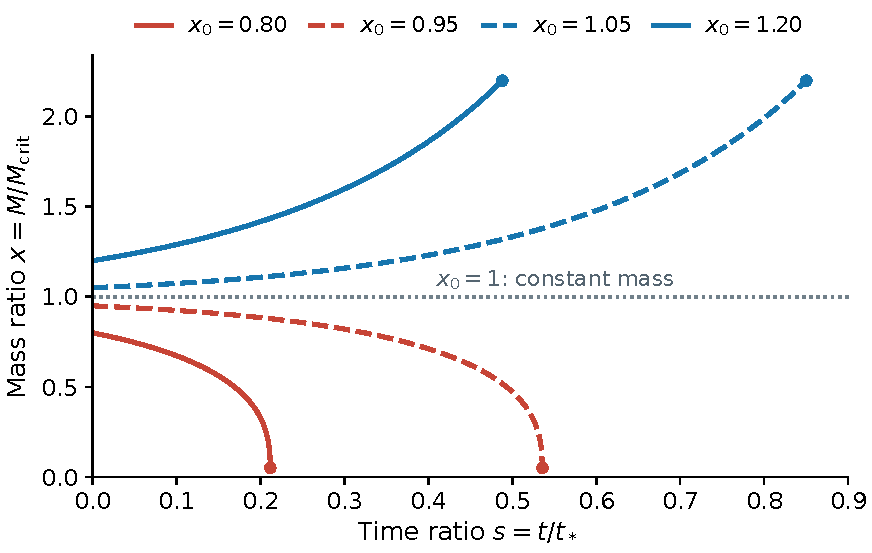
\includegraphics[width=.82\linewidth]{figure2.pdf}
 \caption{\textbf{Perturbations move away from the fixed-medium balance on both sides.} Red curves start below $\Mcrit$ and blue curves above it; dashed curves start closer to the balance. Filled dots mark plotting cutoffs. For the reference medium one unit of $s$ is $2.44\times10^8$~yr.}
 \label{fig:fixed-traj}
\end{figure}

\subsection{When can a balance be stable?}
For a general one-variable law $\dot M=C(M)-E(M)$ with positive gain $C$ and loss $E$ balancing at $M_*$, where $C(M_*)=E(M_*)=R_*$,
\begin{equation*}
 \left.\frac{d\dot M}{dM}\right|_{M_*}=\frac{R_*}{M_*}(p-q),\qquad
 p=\frac{d\ln C}{d\ln M},\quad q=\frac{d\ln E}{d\ln M}.
\end{equation*}
A balance is stable only if the gain rises more slowly with mass than the loss, $p<q$. Bondi accretion and Hawking evaporation give $p=2$ and $q=-2$, the opposite. Within a one-variable description, no choice of medium can change these exponents. A stable balance would therefore need an additional variable that responds to the hole, and the most direct candidate is the temperature of the gas it heats.

\section{Thermal feedback model}\label{sec:model}
\subsection{Temperature-dependent accretion}
At balance, the reference hole of Sec.~\ref{sec:fixed} radiates $\Pbb(\Mcrit)=3.6\times10^{11}$~W into a medium assumed to stay unchanged. For an ideal gas with fixed composition, $c_s^2=\gamma k_BT/(\mu m_p)$, so at fixed $\rho_\infty$ and $\lambda$ Eq.~\eqref{eq:bondi} becomes
\begin{equation}
 A(T)=A_0\left(\frac{T}{T_0}\right)^{-3/2}.
 \label{eq:AT}
\end{equation}
The temperature $T$ must describe the gas that sets the Bondi boundary condition, at radii of order $r_B$ and beyond; heating only a thin layer near the horizon would not change it. We therefore assume a well-mixed reservoir in which deposited radiation reaches the gas that controls accretion. This closure is tested in Sec.~\ref{sec:physical}.

\subsection{Heating and cooling}
Let a fraction $\epsilon$ of the blackbody luminosity heat a reservoir of constant heat capacity $\Cenv$, and let linear cooling return it to $T_0$ on a timescale $\tau_c$:
\begin{equation}
 \dot M=A_0\left(\frac{T}{T_0}\right)^{-3/2}M^2-\frac{B}{M^2},\qquad
 \Cenv\dot T=\frac{\epsilon K}{M^2}-\frac{\Cenv}{\tau_c}(T-T_0),
 \label{eq:dimensional}
\end{equation}
with all constants positive and $0<\epsilon\le1$. The parameters $\epsilon$, $\Cenv$ and $\tau_c$ are not derived from the emission spectrum, opacity or geometry, and the reservoir neither has spatial structure nor tracks the energy carried by gas flowing in and out.

\subsection{The feedback loop}
Equation~\eqref{eq:dimensional} contains a single closed loop (Fig.~\ref{fig:loop}). A decrease of $M$ raises $\Pbb$; the deposited power heats the reservoir; the higher sound speed lowers $A(T)$; and the weaker accretion lets evaporation remove mass faster. Holding $\rho_\infty$ fixed isolates this sound-speed channel; the response of the density and the transport delay between the deposition region and the Bondi radius are not modeled.

\begin{figure}[tbp]
\centering
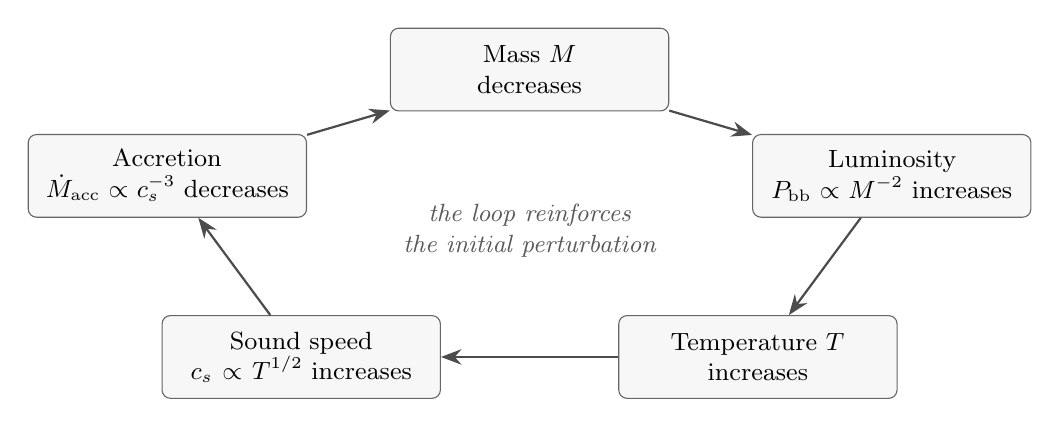
\begin{tikzpicture}[
  box/.style={draw=black!60, rounded corners=3pt, fill=black!3, align=center,
              text width=3.3cm, minimum height=1.05cm, font=\small},
  arr/.style={-{Stealth[length=2.6mm]}, thick, black!70}]
 \node[box] (m) at (0,1.9)     {Mass $M$\\decreases};
 \node[box] (p) at (4.6,0.55)  {Luminosity\\$\Pbb\propto M^{-2}$ increases};
 \node[box] (t) at (2.9,-1.75) {Temperature $T$\\increases};
 \node[box] (c) at (-2.9,-1.75){Sound speed\\$c_s\propto T^{1/2}$ increases};
 \node[box] (a) at (-4.6,0.55) {Accretion\\$\dot M_{\rm acc}\propto c_s^{-3}$ decreases};
 \draw[arr] (m) -- (p);
 \draw[arr] (p) -- (t);
 \draw[arr] (t) -- (c);
 \draw[arr] (c) -- (a);
 \draw[arr] (a) -- (m);
 \node[font=\small\itshape, text=black!65, align=center] at (0,-0.15) {the loop reinforces\\the initial perturbation};
\end{tikzpicture}
\caption{\textbf{The thermal feedback loop for a downward mass perturbation.} Every link follows from Eq.~\eqref{eq:dimensional}. An upward perturbation runs the same loop with every change reversed and favors further growth.}
\label{fig:loop}
\end{figure}

\subsection{Dimensionless form}
Let $\Mc=(B/A_0)^{1/4}$ be the fixed-medium balance mass, Eq.~\eqref{eq:mcrit}, at $T=T_0$, and $\tstar=(A_0\Mc)^{-1}$ its time unit. With $x=M/\Mc$, $\theta=T/T_0$ and $s=t/\tstar$, Eq.~\eqref{eq:dimensional} becomes
\begin{equation}
 \frac{dx}{ds}=F(x,\theta)=\theta^{-3/2}x^2-x^{-2},\qquad
 \frac{d\theta}{ds}=G(x,\theta)=\eta x^{-2}-\zeta(\theta-1),
 \label{eq:system}
\end{equation}
where
\begin{equation}
 \eta=\frac{\tstar\epsilon K}{\Cenv T_0\Mc^2},\qquad
 \zeta=\frac{\tstar}{\tau_c},\qquad
 \chi=\frac{\eta}{\zeta}=\frac{\epsilon\Pbb(\Mc)\,\tau_c}{\Cenv T_0}.
 \label{eq:params}
\end{equation}
The feedback strength $\chi$ compares the energy deposited during one cooling time with the thermal energy scale $\Cenv T_0$ of the reservoir; the cooling rate $\zeta$ compares the cooling time with the mass time unit. For $\eta=0$ the temperature stays at $\theta=1$ and Eq.~\eqref{eq:system} reduces to Eq.~\eqref{eq:dimensionless}.

\section{Equilibrium and stability with feedback}\label{sec:stability}
\subsection{The shifted equilibrium}
The nullclines of Eq.~\eqref{eq:system} are $x=\theta^{3/8}$ ($F=0$) and $\theta=1+\chi x^{-2}$ ($G=0$). The first rises with temperature and the second falls with mass, so they intersect once, at
\begin{equation}
 x_*=\theta_*^{3/8},\qquad \theta_*-1=\chi\,\theta_*^{-3/4}.
 \label{eq:equilibrium}
\end{equation}
The function $h(\theta)=\theta-1-\chi\theta^{-3/4}$ is negative at $\theta=1$, grows without bound, and has $h'>0$, so for every $\chi>0$ there is exactly one positive equilibrium, with $\theta_*>1$ and $x_*>1$. For weak feedback $\theta_*=1+\chi+O(\chi^2)$ and $x_*=1+\tfrac38\chi+O(\chi^2)$; for strong feedback $\theta_*\sim\chi^{4/7}$ and $x_*\sim\chi^{3/14}$. Heating therefore moves the balance to a hotter medium and a larger mass (Fig.~\ref{fig:equilibrium}a). Whether trajectories return to it is a separate question.

\begin{figure}[tbp]
 \centering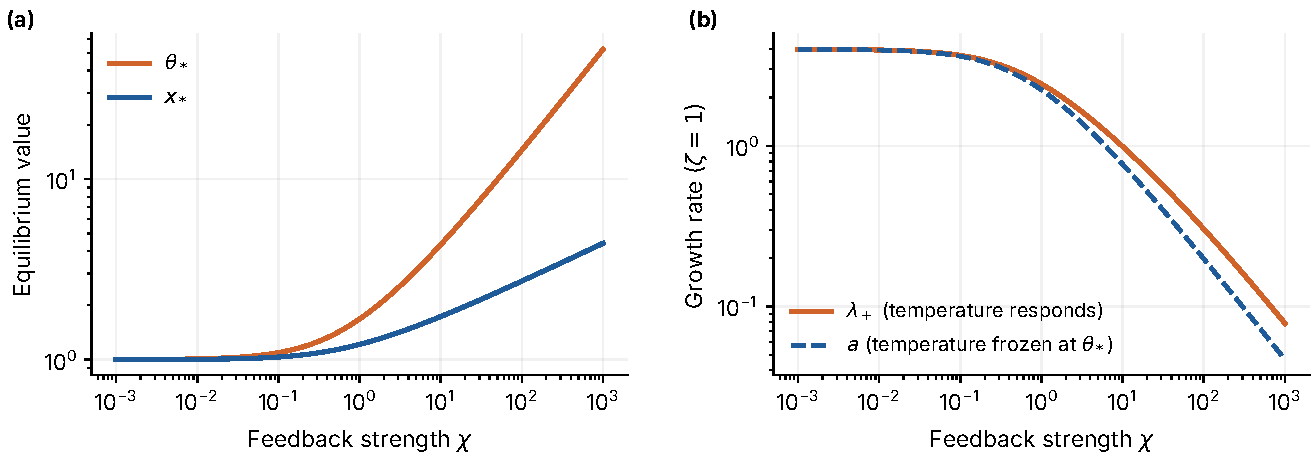
\includegraphics[width=\linewidth]{equilibrium.pdf}
 \caption{\textbf{Heating shifts the balance without making it attracting.} (a) Equilibrium temperature and mass from Eq.~\eqref{eq:equilibrium}. (b) For $\zeta=1$, the unstable eigenvalue $\lambda_+$ of the coupled system and the growth rate $a=4x_*^{-3}$ obtained when the temperature is frozen at $\theta_*$. Both rates fall as the equilibrium moves to larger mass, but $\lambda_+>a$ throughout.}
 \label{fig:equilibrium}
\end{figure}

\subsection{A saddle for every positive coupling}
The partial derivatives of Eq.~\eqref{eq:system} are $F_x=2\theta^{-3/2}x+2x^{-3}$, $F_\theta=-\tfrac32\theta^{-5/2}x^2$, $G_x=-2\eta x^{-3}$ and $G_\theta=-\zeta$. At the equilibrium $\theta_*^{-3/2}=x_*^{-4}$, so the Jacobian is
\begin{equation*}
 J_*=\begin{pmatrix} a & b\\ c & -\zeta\end{pmatrix},\qquad
 a=4x_*^{-3}>0,\quad
 b=-\tfrac32\theta_*^{-5/2}x_*^2<0,\quad
 c=-2\eta x_*^{-3}<0,
\end{equation*}
with determinant
\begin{equation}
 \det J_*=-4\zeta x_*^{-3}-3\eta\,\theta_*^{-5/2}x_*^{-1}<0.
 \label{eq:det}
\end{equation}
A real $2\times2$ matrix with negative determinant has two real eigenvalues of opposite sign. The equilibrium is therefore a saddle for every $\eta,\zeta>0$. A stable node, a stable focus and a Hopf bifurcation are all excluded, because each requires $\det J_*>0$.

\subsection{Three growth rates}
Three rates are easily confused when judging the effect of heating: the rate $a$ of a mass perturbation at the new equilibrium with the temperature frozen at $\theta_*$; the unstable eigenvalue of the coupled system,
\begin{equation}
 \lambda_\pm=\frac{a-\zeta\pm\sqrt{(a+\zeta)^2+4bc}}{2},\qquad
 \lambda_+>a>0,\qquad \lambda_-<-\zeta,
 \label{eq:eigenvalues}
\end{equation}
where the inequalities follow from $bc>0$; and the rate 4 of the fixed-medium balance. For $\chi=\zeta=1$ these are $a=2.234$, $\lambda_+=2.431$ and 4. Letting the temperature respond raises the growth rate at a given equilibrium from $a$ to $\lambda_+$, so the coupling itself is destabilizing. The shift of the equilibrium to larger mass lowers all rates, which is why $\lambda_+$ is smaller than 4; this reflects the new equilibrium, not a stabilizing effect.

The unstable eigenvector has slope $(\lambda_+-a)/b<0$ in the $(x,\theta)$ plane and the stable one has slope $(\lambda_--a)/b>0$. Only initial conditions on the one-dimensional stable manifold approach the equilibrium. For fixed $\zeta$ and $\chi\gg1$, $\lambda_+\sim7\chi^{-9/14}$ (Appendix~\ref{app:scaling}): the growth rate becomes small but stays positive for every finite $\chi$. At fixed $\chi$, the slow- and fast-cooling limits are
\begin{equation*}
 \lim_{\zeta\to0^+}\lambda_+=a,\qquad
 \lim_{\zeta\to\infty}\lambda_+=a+3\chi\,\theta_*^{-5/2}x_*^{-1}>a.
\end{equation*}
In the first limit the temperature cannot respond during a mass e-folding; in the second it follows the mass along $G=0$. Neither limit reverses the instability.

\subsection{A sign theorem}
The saddle does not depend on the specific power laws or on linear cooling.

\begin{proposition}\label{prop:sign}
Consider the one-zone system
\begin{equation*}
 \dot M=\mathcal F(M,T)=A(T)M^2-BM^{-2},\qquad
 \dot T=\mathcal G(M,T)=H(M)-\Lambda(T),
\end{equation*}
with $B>0$ and differentiable $A$, $H$, $\Lambda$. If at a positive equilibrium $A>0$, $A'(T)<0$, $H'(M)<0$ and $\Lambda'(T)>0$, that equilibrium is a saddle.
\end{proposition}
\begin{proof}
At the equilibrium, $\mathcal F_M=2AM+2BM^{-3}>0$, $\mathcal F_T=A'M^2<0$, $\mathcal G_M=H'<0$ and $\mathcal G_T=-\Lambda'<0$. Hence $\det D(\mathcal F,\mathcal G)=\mathcal F_M\mathcal G_T-\mathcal F_T\mathcal G_M<0$.
\end{proof}

The three conditions have direct physical meanings: hotter gas accretes less efficiently, a lighter hole heats its surroundings more strongly, and a hotter reservoir cools faster. They also cover a medium held at fixed pressure rather than fixed density: then $\rho_\infty\propto T^{-1}$ and $A\propto T^{-5/2}$, which still decreases with temperature. Stabilization within a one-zone description would require reversing one of these signs. A model with additional state variables, such as an independently evolving density, is not covered by the proposition, and its stability has to be determined from its own Jacobian.

\section{Numerical checks of the coupled model}\label{sec:numerics}
We solve Eq.~\eqref{eq:equilibrium} with a bracketed root finder, evaluate $J_*$ analytically, and integrate Eq.~\eqref{eq:system} with the same solver as in Sec.~\ref{sec:fixed} and a maximum step of 0.01. For $\chi=\zeta=1$,
\begin{equation*}
 (x_*,\theta_*)=(1.214276,\,1.678211),\qquad (\lambda_-,\lambda_+)=(-1.197336,\,2.431462).
\end{equation*}
Table~\ref{tab:scan} lists the equilibrium and the rates for five feedback strengths. In every row $\lambda_+>a>0$, while both rates decrease as the equilibrium moves to larger mass.

\begin{table}[tbp]
\centering\small
\caption{Equilibria, growth rates and Jacobian determinants for $\zeta=1$. The rate $a$ freezes the temperature at $\theta_*$; $\lambda_\pm$ include the temperature response. All quantities are dimensionless.}
\label{tab:scan}
\begin{tabular}{@{}rrrrrrr@{}}
\toprule
$\chi$ & $\theta_*$ & $x_*$ & $a$ & $\lambda_-$ & $\lambda_+$ & $\det J_*$\\
\midrule
0.01 & 1.00993 & 1.00371 & 3.95580 & $-1.00588$ & 3.96168 & $-3.98496$\\
0.1 & 1.09352 & 1.03409 & 3.61728 & $-1.04971$ & 3.66699 & $-3.84929$\\
1 & 1.67821 & 1.21428 & 2.23413 & $-1.19734$ & 2.43146 & $-2.91128$\\
10 & 4.33092 & 1.73268 & 0.76897 & $-1.22271$ & 0.99167 & $-1.21253$\\
100 & 14.47513 & 2.72417 & 0.19786 & $-1.10595$ & 0.30381 & $-0.33600$\\
\bottomrule
\end{tabular}
\end{table}

Figure~\ref{fig:phase} shows the nullclines and the manifolds of the saddle for $\chi=\zeta=1$, integrated from displacements of $10^{-6}$ along the eigenvectors. Trajectories to the right of the stable manifold gain mass and those to its left lose it. Figure~\ref{fig:scan} shows $\lambda_+$ on a $201\times201$ logarithmic grid with $10^{-2}\le\chi,\zeta\le10^2$; it ranges from 0.20 to 3.98 and depends mainly on $\chi$, which sets the equilibrium mass. On a separate $41\times41$ grid the code also confirms $\det J_*<0$, $\lambda_+>a>0$ and $\lambda_-<-\zeta$ at every point. These scans illustrate Eq.~\eqref{eq:det}; the analytic determinant establishes the result for all positive parameters.

\begin{figure}[tbp]
 \centering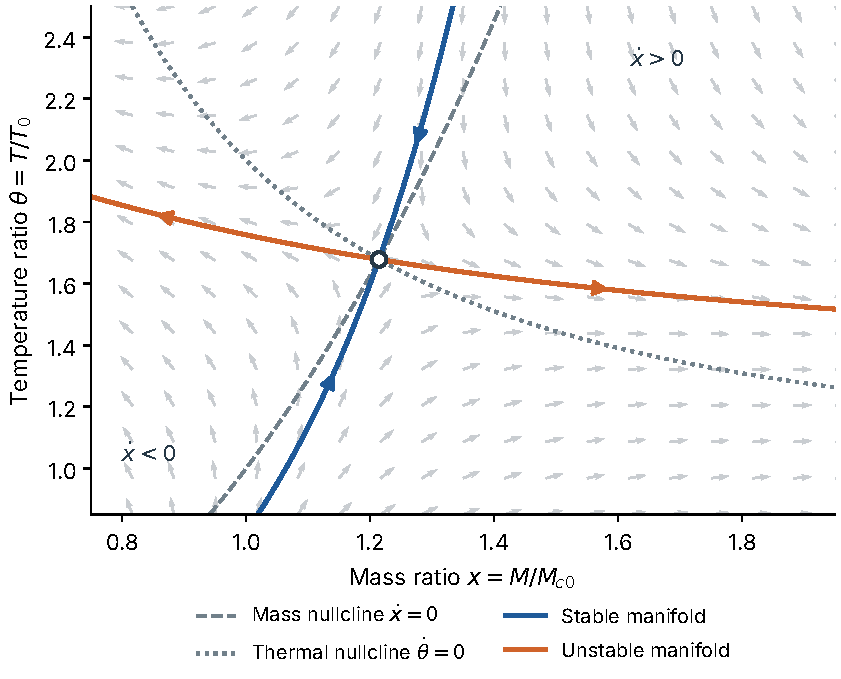
\includegraphics[width=.74\linewidth]{phase_portrait.pdf}
 \caption{\textbf{Phase portrait for $\chi=\zeta=1$.} The mass and thermal nullclines meet at the single equilibrium (open circle). Arrowheads mark the direction of time: the stable manifold (blue) approaches the saddle and the unstable manifold (orange) leaves it. Gray arrows show the direction of the flow.}
 \label{fig:phase}
\end{figure}

\begin{figure}[tbp]
 \centering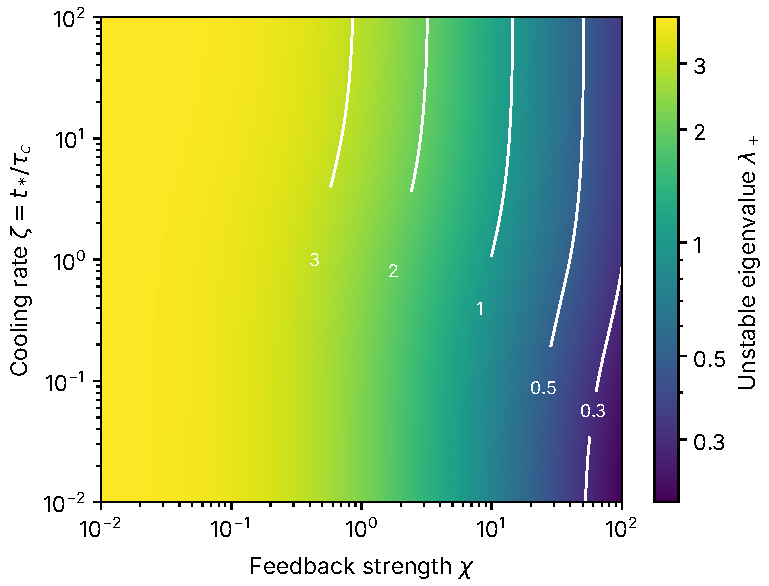
\includegraphics[width=.62\linewidth]{parameter_scan.pdf}
 \caption{\textbf{The unstable eigenvalue over the $(\chi,\zeta)$ plane.} White contours mark constant $\lambda_+$. The eigenvalue decreases with feedback strength but is positive everywhere, as Eq.~\eqref{eq:det} requires.}
 \label{fig:scan}
\end{figure}

Finally, Fig.~\ref{fig:departures} compares the two models directly. Each is perturbed by $\pm2\%$ in mass relative to its own equilibrium: the fixed-medium model from $x=1\pm0.02$ and the coupled model from $(x_*(1\pm0.02),\theta_*)$. All four trajectories leave their balance. The coupled ones leave more slowly because the equilibrium mass is larger, in agreement with $\lambda_+<4$.

\begin{figure}[tbp]
 \centering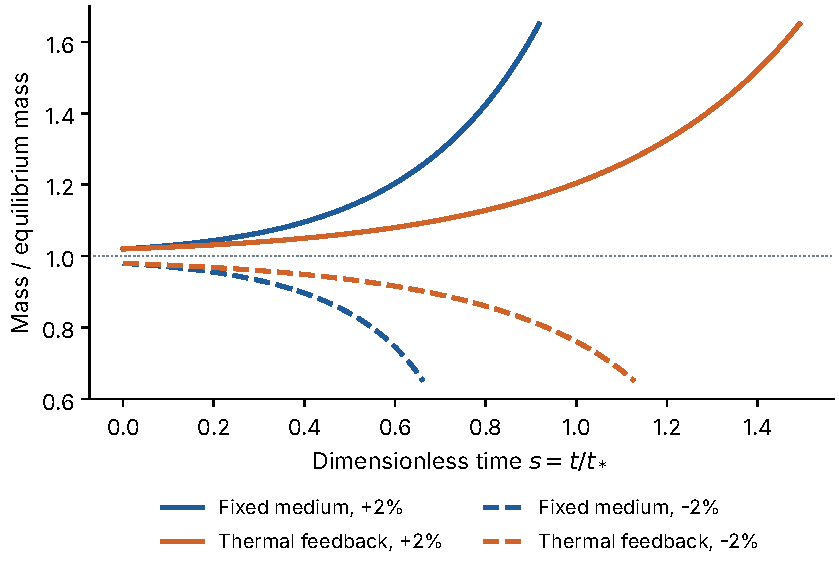
\includegraphics[width=.74\linewidth]{departures.pdf}
 \caption{\textbf{Both balances repel perturbations.} Mass divided by each model's own equilibrium mass after $\pm2\%$ perturbations; the coupled model has $\chi=\zeta=1$ and starts at its equilibrium temperature. Curves end at plotting cutoffs.}
 \label{fig:departures}
\end{figure}

\section{Physical scales}\label{sec:physical}
The saddle result does not depend on material constants, but identifying $T$ with the temperature that sets the Bondi boundary condition does. We test this identification with two fully ionized hydrogen media: a hot plasma with $T_0=10^6$~K and proton density $n=10^{20}\,\mathrm{m^{-3}}$, and a hydrogen medium at the central temperature and density of the Sun, $T_0=1.56\times10^7$~K and $\rho=1.5\times10^5\,\mathrm{kg\,m^{-3}}$~\cite{nasa}. The second case borrows only these two numbers and is not a model of the solar core. In both, $\gamma=5/3$, $\mu=1/2$ and $\lambda=1/4$.

\subsection{Flow, heating and cooling times}
At the balance mass $\Mc$ we define the Bondi radius $r_B=G\Mc/c_s^2$ and the flow time $t_{\rm flow}=r_B/c_s$. A sphere of radius $r_B$ contains thermal energy $E_B=3nk_BT_0V_B$, with $V_B=4\pi r_B^3/3$. The Thomson optical depth $\tau_T=n\sigma_Tr_B$ estimates the probability that a photon scatters once while crossing it. If every scattered photon gave all of its energy to the gas, the heating rate would be $\tau_T\Pbb(\Mc)$, giving the shortest possible photon heating time
\begin{equation*}
 t_{{\rm heat},T}=\frac{E_B}{\tau_T\Pbb(\Mc)}.
\end{equation*}
In reality a scattering transfers only part of the photon energy, the cross section falls below the Thomson value at high energy, and other Hawking particles are not included in this estimate. For cooling we use optically thin free--free emission of pure hydrogen from the NRL Plasma Formulary~\cite{nrl},
\begin{equation*}
 q_{\rm ff}=1.69\times10^{-38}\,n^2\sqrt{k_BT_0/(1\,{\rm eV})}\ \mathrm{W\,m^{-3}},\qquad
 t_{\rm ff}=\frac{3nk_BT_0}{q_{\rm ff}},
\end{equation*}
with $n$ in $\mathrm{m^{-3}}$. The ion mean free path $\ell_{ii}=v_{Ti}/\nu_{ii}$ uses the NRL thermal speed $v_{Ti}=(k_BT/m_p)^{1/2}$ and ion collision rate with $\ln\Lambda=10$. Table~\ref{tab:plasma} collects the results.

\begin{table}[tbp]
\centering\small
\caption{Order-of-magnitude scales at the fixed-medium balance mass $\Mc$ for two fully ionized hydrogen media. Only $T_0$ and $n$ are inputs; the other entries follow from the blackbody, Thomson, free--free and NRL collision prescriptions in the text.}
\label{tab:plasma}
\begin{tabular}{@{}lrr@{}}
\toprule
Quantity & Hot plasma & Solar-center hydrogen\\
\midrule
$T_0$ (K) & $1.00\times10^{6}$ & $1.56\times10^{7}$\\
$n$ ($\mathrm{m^{-3}}$) & $1.00\times10^{20}$ & $8.97\times10^{31}$\\
$c_s$ ($\mathrm{m\,s^{-1}}$) & $1.66\times10^{5}$ & $6.55\times10^{5}$\\
$\Mc$ (kg) & $2.96\times10^{14}$ & $8.54\times10^{11}$\\
$r_B$ (m) & $7.19\times10^{-7}$ & $1.33\times10^{-10}$\\
$t_{\rm flow}$ (s) & $4.34\times10^{-12}$ & $2.03\times10^{-16}$\\
$\tau_T$ & $4.78\times10^{-15}$ & $7.92\times10^{-7}$\\
$\tau_T\Pbb(\Mc)$ (W) & $1.94\times10^{-11}$ & $3.87\times10^{2}$\\
$t_{{\rm heat},T}$ (s) & $3.33\times10^{-4}$ & $1.47\times10^{-15}$\\
$t_{\rm ff}$ (s) & $2.64$ & $1.16\times10^{-11}$\\
$\ell_{ii}/r_B$ & $2.1\times10^{6}$ & $3.1$\\
\bottomrule
\end{tabular}
\end{table}

In the hot plasma, $t_{{\rm heat},T}/t_{\rm flow}\simeq7.7\times10^7$; in the denser medium the ratio is still about 7. Free--free cooling is slower than the flow by factors of $6.1\times10^{11}$ and $5.7\times10^4$. Gas therefore crosses the Bondi region long before it is heated or cools radiatively. If the exchange of gas relaxes the reservoir on $\tau_c\sim t_{\rm flow}$, Eq.~\eqref{eq:params} gives photon-only estimates $\chi\approx1.3\times10^{-8}$ and $0.14$, both upper limits. In addition, the ion mean free path exceeds $r_B$ in both media, so even the continuum Bondi flow assumed at the balance mass is not established. The denser case is sensitive to composition, collision physics and the non-blackbody Hawking spectrum, so its numbers are diagnostics, not statements about the Sun.

\subsection{Radiation pressure}
Radiation can also push the gas away rather than heat it. For a luminosity $L$ and a flux-mean opacity $\kappa_F$, radiation pressure balances gravity at the Eddington luminosity $L_E=4\pi GMc/\kappa_F$. Inserting $L=\Pbb=K/M^2$ gives a force ratio
\begin{equation*}
 \frac{a_{\rm rad}}{a_{\rm grav}}=\left(\frac{M_E}{M}\right)^3,\qquad
 M_E=\left(\frac{\kappa_FK}{4\pi Gc}\right)^{1/3}.
\end{equation*}
For the Thomson opacity of ionized hydrogen, $\kappa_F=\sigma_T/m_p$, this gives $M_E=3.8\times10^{10}$~kg. The ratio is $5.6\times10^{10}$ at the reference mass $M_0$, so a hole of that mass would blow away rather than accrete optically coupled gas. At the balance masses of Table~\ref{tab:plasma} it is only $2\times10^{-12}$ and $9\times10^{-5}$, and radiation pressure does not prevent accretion there. Applying a low-energy opacity to a TeV-scale, multispecies spectrum is itself a rough approximation~\cite{ciotti}.

\subsection{Relation to accretion-powered feedback}
Cantiello et al.~\cite{cantiello} solve time-dependent spherical hydrodynamics with radiative cooling for primordial black holes in stellar cores. They identify a hot-Bondi regime, a bremsstrahlung-cooling regime that drives the flow toward isothermal, and a photon-trapping regime, and find that cooling raises the accretion rate by a factor of about 2--7 relative to adiabatic Bondi. Their black hole has no intrinsic luminosity; the radiation comes from the accreting gas.

This difference reverses the sign of the feedback. In an accretion-powered system, a higher accretion rate produces more radiation and more heating, which then limits accretion: the feedback is negative and tends to regulate the flow. A Hawking-powered hole radiates more when its mass decreases, so the same thermal suppression of accretion acts in the direction of the original perturbation. This reversal is the physical origin of the saddle. For the same reason, their quantitative results cannot be used to fix $\epsilon$, $\Cenv$ or $\tau_c$ here.

\subsection{Toward a physical model}
Connecting Eq.~\eqref{eq:system} to a real medium would require a collisional mean free path much smaller than $r_B$; heating and thermalization fast enough to change the sound speed at the Bondi radius; a deposition calculation for the actual Hawking spectrum; and an energy budget that includes advection, radiation and density evolution. The illustrative choice $\chi=\zeta=1$ in Sec.~\ref{sec:numerics} is not a calibration of either medium in Table~\ref{tab:plasma}. These requirements suggest a hierarchy of models in which each step adds one physical ingredient (Table~\ref{tab:hierarchy}). The next step, a density response, adds a third state variable. Proposition~\ref{prop:sign} does not apply to it, so its stability has to be tested anew.

\begin{table}[tbp]
\centering\small
\caption{A hierarchy of Hawking--Bondi models.}
\label{tab:hierarchy}
\begin{tabular}{@{}lll@{}}
\toprule
Model & State variables & Accretion law\\
\midrule
Fixed medium, Sec.~\ref{sec:fixed} & $M$ & $A=\text{const}$\\
Thermal feedback, Secs.~\ref{sec:model}--\ref{sec:numerics} & $M,\,T$ & $A(T)$\\
Density response & $M,\,T,\,\rho$ & $A(T,\rho)$\\
Radiation hydrodynamics & $M,\,\rho(r),\,T(r),\,v(r)$ & solved from the flow\\
\bottomrule
\end{tabular}
\end{table}

\section{Conclusion}
In a fixed medium, Bondi accretion and blackbody Hawking evaporation balance at exactly one mass, and that balance is unstable: the gain grows with mass while the loss falls. The exact solution shows that evaporation far below the balance is fast, while departures from a nearly balanced state can take hundreds of millions of years for the reference medium.

Letting the hole's radiation heat the medium does not rescue the balance. The coupled mass--temperature system has a single equilibrium, hotter and more massive than the fixed-medium one, and its Jacobian determinant is negative for all positive feedback and cooling strengths, so the equilibrium is a saddle. The same holds for every one-zone model in which heating decreases with mass, accretion decreases with temperature and cooling increases with temperature. The thermal response is destabilizing: at a given equilibrium it raises the growth rate from $a$ to $\lambda_+$. The physical reason is the sign of the loop: a Hawking-powered hole radiates more as it loses mass, so heating suppresses accretion exactly when accretion is needed.

Timescale estimates for two hydrogen plasmas show that gas crosses the Bondi region faster than it heats or cools, so neither supports a one-zone thermal reservoir at its balance mass. Whether density evolution, spatial transport or realistic emission spectra can change the result remains open; the sign conditions of Proposition~\ref{prop:sign} identify what any such extension must check.

\section*{Acknowledgments}
I thank Hadi Erturk (University of Oxford) for mentoring this project and for helpful suggestions throughout. I also thank Ore Gottlieb (MIT) for reading an early version of the fixed-medium analysis, for his encouraging comments on its physical intuition, and for motivating the thermal-feedback extension developed here.

\appendix
\section{The coefficient in the Hawking temperature}\label{app:temperature}
We use the regular Euclidean Schwarzschild geometry to recover the coefficient in Eq.~\eqref{eq:temperature}~\cite{gibbons,genolini}. The Lorentzian line element is
\begin{equation*}
 d\ell^2=-f(r)c^2dt^2+\frac{dr^2}{f(r)}+r^2d\Omega^2,
 \qquad f(r)=1-\frac{r_s}{r}.
\end{equation*}
After continuing $t=-it_E$, set $r=r_s+\varepsilon$ near the horizon and define $R=2\sqrt{r_s\varepsilon}$. To leading order in $\varepsilon/r_s$,
\begin{equation*}
 f\simeq\frac{R^2}{4r_s^2},\qquad
 \frac{dr^2}{f}\simeq dR^2,\qquad
 d\ell_E^2\simeq dR^2+R^2d\varphi^2,
 \qquad\varphi=\frac{ct_E}{2r_s}.
\end{equation*}
For this plane to be smooth at $R=0$, $\varphi$ must have period $2\pi$, so $t_E$ has period $\Delta t_E=4\pi r_s/c=8\pi GM/c^3$. A thermal state has imaginary-time period $\hbar/(k_BT_H)$, which gives $T_H=\hbar c^3/(8\pi GMk_B)$. This argument fixes the temperature but not the emitted flux, which requires a quantum-field and greybody calculation~\cite{hawking,page}.

\section{The strong-feedback limit}\label{app:scaling}
At $\Mc$, $B=A_0\Mc^4$ and $\tstar^{-1}=A_0\Mc$; substituting $M=\Mc x$, $T=T_0\theta$ and $t=\tstar s$ into Eq.~\eqref{eq:dimensional} gives Eq.~\eqref{eq:system}. For $\chi\gg1$, Eq.~\eqref{eq:equilibrium} gives $\theta_*^{7/4}\sim\chi$ and $x_*\sim\chi^{3/14}$, hence $a=4x_*^{-3}\sim4\chi^{-9/14}$ and $bc=3\eta\,\theta_*^{-5/2}x_*^{-1}\sim3\zeta\chi^{-9/14}$. At fixed $\zeta$, $a\to0$ and the positive root of Eq.~\eqref{eq:eigenvalues} behaves as $\lambda_+\sim a+bc/\zeta\sim7\chi^{-9/14}$. This limit is not uniform if $\zeta$ also tends to zero.

\section{Reference values and reproducibility}\label{app:values}
We use SI values $G=6.67430\times10^{-11}\,\mathrm{m^3\,kg^{-1}\,s^{-2}}$, $c=299792458\,\mathrm{m\,s^{-1}}$, $h=6.62607015\times10^{-34}$~J\,s, $k_B=1.380649\times10^{-23}\,\mathrm{J\,K^{-1}}$, $m_p=1.67262192\times10^{-27}$~kg, $\sigma_T=6.6524587\times10^{-29}\,\mathrm{m^2}$ and a year of 365.25 days. Table~\ref{tab:values} lists the fixed-medium reference values.

\begin{table}[htbp]
\centering\small
\caption{Reference values of the blackbody, fixed-medium model.}
\label{tab:values}
\begin{tabular}{@{}lrl@{}}
\toprule
Quantity & Value & Unit\\
\midrule
Reference mass $M_0$ & $1.00\times10^7$ & kg\\
Hawking temperature $T_H(M_0)$ & $1.23\times10^{16}$ & K\\
Blackbody luminosity $\Pbb(M_0)$ & $3.56\times10^{18}$ & W\\
Pure-evaporation lifetime $\taubb(M_0)$ & $23.37$ & h\\
Accretion coefficient $A$ & $4.15\times10^{-27}$ & $\mathrm{kg^{-1}\,s^{-1}}$\\
Evaporation coefficient $B$ & $3.96\times10^{15}$ & $\mathrm{kg^3\,s^{-1}}$\\
Balance mass $\Mcrit$ & $3.13\times10^{10}$ & kg\\
Time unit $\tstar$ & $2.44\times10^8$ & yr\\
Perturbation e-folding time $t_e$ & $6.11\times10^7$ & yr\\
\bottomrule
\end{tabular}
\end{table}

The repository~\cite{repo} contains two scripts. \texttt{paper/reproduce.py} computes the fixed-medium values and Figs.~\ref{fig:fixed-rate}--\ref{fig:fixed-traj}; \texttt{thermal-feedback/reproduce.py} computes Tables~\ref{tab:scan}--\ref{tab:plasma} and Figs.~\ref{fig:equilibrium}--\ref{fig:departures}. Figure~\ref{fig:loop} is drawn in the \LaTeX\ source. Each script checks its own results: the implicit solution against the numerical trajectories, and the sign of the determinant and the eigenvalue inequalities over a parameter grid.

{\raggedright
\begin{thebibliography}{99}
\bibitem{hawking} S. W. Hawking, ``Particle creation by black holes,'' \emph{Communications in Mathematical Physics} \textbf{43}, 199--220 (1975). \href{https://doi.org/10.1007/BF02345020}{doi:10.1007/BF02345020}.
\bibitem{gibbons} G. W. Gibbons and S. W. Hawking, ``Action integrals and partition functions in quantum gravity,'' \emph{Physical Review D} \textbf{15}, 2752--2756 (1977). \href{https://doi.org/10.1103/PhysRevD.15.2752}{doi:10.1103/PhysRevD.15.2752}.
\bibitem{genolini} P. Benetti Genolini, ``Introduction to black hole thermodynamics,'' lecture notes (2025). \href{https://arxiv.org/abs/2512.24929}{arXiv:2512.24929}.
\bibitem{page} D. N. Page, ``Particle emission rates from a black hole: Massless particles from an uncharged, nonrotating hole,'' \emph{Physical Review D} \textbf{13}, 198--206 (1976). \href{https://doi.org/10.1103/PhysRevD.13.198}{doi:10.1103/PhysRevD.13.198}.
\bibitem{macgibbon} J. H. MacGibbon and B. R. Webber, ``Quark- and gluon-jet emission from primordial black holes: The instantaneous spectra,'' \emph{Physical Review D} \textbf{41}, 3052--3079 (1990). \href{https://doi.org/10.1103/PhysRevD.41.3052}{doi:10.1103/PhysRevD.41.3052}.
\bibitem{bondi} H. Bondi, ``On spherically symmetrical accretion,'' \emph{Monthly Notices of the Royal Astronomical Society} \textbf{112}, 195--204 (1952). \href{https://doi.org/10.1093/mnras/112.2.195}{doi:10.1093/mnras/112.2.195}.
\bibitem{cantiello} M. Cantiello, O. Gottlieb, C. Norton, M. Kleban and K. Van Tilburg, ``Accretion of primordial black holes in stellar interiors,'' arXiv preprint (2026). \href{https://arxiv.org/abs/2606.02726}{arXiv:2606.02726}.
\bibitem{nasa} NASA Marshall Space Flight Center, ``The solar interior,'' \url{https://solarscience.msfc.nasa.gov/interior.shtml} (accessed 30 September 2026).
\bibitem{nrl} A. Beresnyak, \emph{NRL Plasma Formulary}, U.S. Naval Research Laboratory (2023).
\bibitem{ciotti} L. Ciotti and J. P. Ostriker, ``Free-free absorption effects on Eddington luminosity,'' (2003). \href{https://arxiv.org/abs/astro-ph/0312490}{arXiv:astro-ph/0312490}.
\bibitem{repo} E. Anaraly uulu, code and manuscripts for this project (2026). \url{https://github.com/IPhO-KG/microscopic-black-hole-reactor}.
\end{thebibliography}
}

\end{document}
